\documentclass[10pt]{article}
\usepackage{amsmath}
\usepackage{paralist}
\usepackage{setspace}
\usepackage{listings}
\usepackage{graphicx}
\usepackage[english]{babel}
\usepackage{geometry}
\usepackage{subcaption}
\usepackage[utf8]{inputenc}
\usepackage{listings}

\begin{document}
\lstset{
	language=Matlab,
	basicstyle=\footnotesize,
	frame=tb,
	xleftmargin=.2\textwidth,
	xrightmargin=.2\textwidth
}
\onehalfspacing
\begin{titlepage}
\begin{center}
% Oberer Teil der Titelseite:


\textsc{\LARGE University Oldenburg}\\[1.5cm]

\textsc{\Large Wind Physics Measurement Project}\\[0.5cm]


% Title
\newcommand{\HRule}{\rule{\linewidth}{0.5mm}}
\HRule \\[0.4cm]
{ \huge \bfseries Exercise 1 - Handling and preprocessing of measurement data}\\[0.4cm]

\HRule \\[1.5cm]

% Author and supervisor
\begin{minipage}{0.4\textwidth}
\begin{flushleft} \large
\emph{Author:}\\
Jan \textsc{K\"amper}\\
Florian \textsc{B\"orgel}
\end{flushleft}
\end{minipage}
\hfill
\begin{minipage}{0.4\textwidth}
\begin{flushright} \large
\emph{Supervisor:} \\
Matthias \textsc{Wächter}
\end{flushright}
\end{minipage}
\\[3cm]
\vfill



% Unterer Teil der Seite
{\large \today}

\end{center}

\end{titlepage}
\tableofcontents
\newpage
\section{Importing Data into Matlab}
For the first task we used the Matlab function readtable() to import the data. We decided to preprocess the data first before saving to the file.
\section{Marking invalid data}
For the invalid data we used the function NaN(). Matlab checks if there is any invalid Data and replaces it with NaN.\\
\begin{lstlisting}
raw_data(raw_data==-999) = NaN(size(raw_data(raw_data==-999)));
\end{lstlisting}
\section{Generating continuous time axis}
To avoid gaps in the time axis we first converted our time t with datenum() to an numeric value. The numeric values represents elapsed time in units of days. After that we multiplied with $24\frac{h}{d}*3600\frac{s}{h}$ to convert days to seconds. 
Next, we created the continuous time axis, by initializing a vector starting with t(1) and ending with t(end). As stepsize we used 1 second. 
Now we filled our new vector with NaN values and overwrote the file with our existing data.\\
\begin{lstlisting}
disp('Creating continous time axis')
tnew=[t(1):1:t(end)]';
data_pp = NaN(length(tnew),10);
disp('Writing preprocessed Data...')
for i = 1:length(raw_data(:,1))
    data_pp(t(i)-t(1)+1, :) = raw_data(i, :);
end
time = (1:length(data_pp))';
data_pp = [time, data_pp];
save('data_pp.mat', 'data_pp', 'raw_data');
clear;
\end{lstlisting}
\section{Computing 10min means and stddev}
\begin{figure}[htb!]
  \centering
  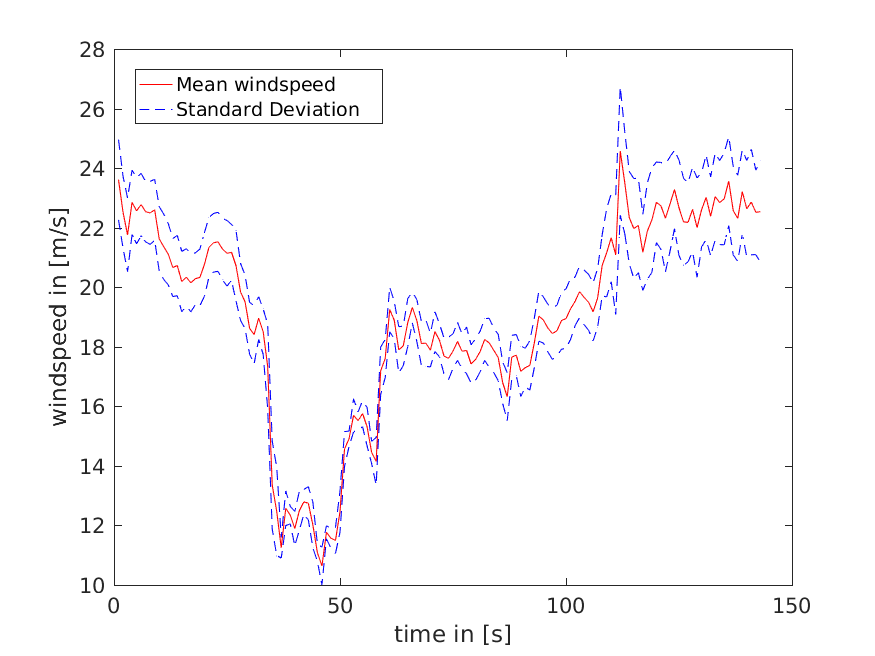
\includegraphics[width=1\linewidth]{../Plots/mean_intervall_withstd.png}
  \caption{10 minute intervalls}\end{figure}
\end{document}
